% !TEX root = ../build-polygon/proof-recursion.tex

\section{Appendix: Proof Composition with SNARKjs and PIL-STARK}

In this section, we are going to show the current proving capabilities of the \texttt{SNARKjs} and \texttt{PIL-STARK} tool stack. In particular, we are going to see how some cases of proof composition can be achieved, extending the power of both \texttt{SNARKjs} and \texttt{PIL-STARK} beyond what they were originally defined for.

In every case throughout this section we are going to be proving the following statement:
\begin{center}
    ``I known a (secret) value $a_1 = 1$ such that the $(2^5+1 =)$ $33$-th element of the Fibonacci sequence on (public) input $a_0 = 1$ and $a_1$ is equal to $3524578$.''
\end{center} 

In the first two sections, we recall the workflow that needs to be followed to generate a (depth $0$) proof.


%%%%%%%%%%%%%%%%%%%%%%%%%%%%%%%%%%%%%%%%%%%%%%%%%%%%%%
\subsection{Depth 0: Circom + SNARKjs}

We represent the statement in Circom, which means that we must represent the computation of the Fibonacci sequence in R1CS format:

\begin{figure}[H]
\centering
% \hspace{-2cm}
\begin{subfigure}[T]{0.5\textwidth}
\begin{circom}
pragma circom 2.1.5;

template Fibonacci(n) {
    signal input a0;
    signal input a1;
    signal output out;

    signal im[n-1];

    for (var i=0; i<n-1; i++) {
        if (i==0) {
            im[i] <== a0 + a1;
        } else if (i==1) {
            im[i] <== a1 + im[0];
        } else {
            im[i] <== im[i-2] + im[i-1];
        }
    }

    out <== im[n-2];
    log("out =", out);
}

component main {public [a0]} = Fibonacci(2**5);
\end{circom}
\end{subfigure}
% \hfill
\begin{subfigure}[T]{0.4\textwidth}
    \centering
    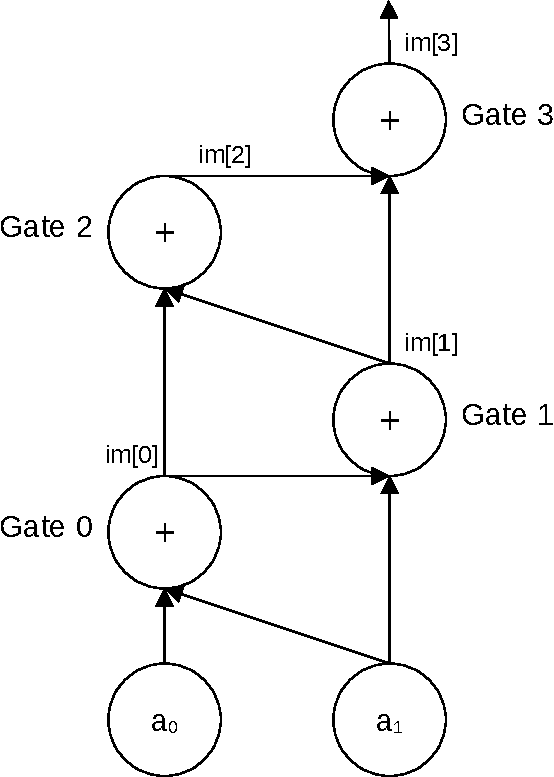
\includegraphics[width=.9\textwidth]{\recursiondir/figures/fibonacci-circuit}
\end{subfigure}
\caption{Circom code for the Fibonacci sequence and the equivalent representation as an arithmetic circuit.}
% \label{fig:STARK-vanilla}
\end{figure}

The execution trace for the particular instance of this circuit (i.e., $a_0 = 1$ and $a_1 = 1$) is as follows:
\[
\begin{array}{|c|c|c|c|}
\hline
\multicolumn{4}{|c|}{\textbf{Execution Trace}} \\\hline
\textbf{Gate 0} & {\color{green!50!black} 1} & {\color{red} 1} & {\color{red} 2} \\\hline
\textbf{Gate 1} & {\color{red} 1} & {\color{red} 2} & {\color{red} 3} \\\hline
\textbf{Gate 2} & {\color{red} 2} & {\color{red} 3} & {\color{red} 5} \\\hline
\vdots & \vdots & \vdots & \vdots \\\hline
\textbf{Gate 32} & {\color{red} 1346269} & {\color{red} 2178309} & {\color{green!50!black} 3524578} \\
\hline
\end{array}
\]
where the numbers colored in red are the information known by the prover, while the numbers colored in green are the information known to both the prover and the verifier.

After the description of the circuit in Circom we can proceed to generate a valid zk-SNARK\footnote{We are going to use PlonK for simplicity, but \texttt{SNARKjs} also supports Groth16 and Fflonk.} for this particular instance using \texttt{SNARKjs}:
\begin{enumerate}
\item Compile the circuit:
\begin{lstlisting}[style=termt]
$ mkdir -p build && circom src/fibonacci.circom --r1cs --wasm -o build

template instances: 1
non-linear constraints: 0
linear constraints: 0
public inputs: 1
public outputs: 1
private inputs: 1
private outputs: 0
wires: 3
labels: 35
\end{lstlisting}

\item Create a \texttt{input.json} file with the inputs for our circuit in the same directory:
\begin{lstlisting}[style=termt]
$ cat <<EOT > input.json
  {"a0": 1, "a1": 1}
  EOT
\end{lstlisting}

\item Compute the witness for our inputs:
\begin{lstlisting}[style=termt]
$ snarkjs wc build/fibonacci_js/fibonacci.wasm src/input.json build/fibonacci.wtns

out = 3524578
\end{lstlisting}

\item Download a sufficiently large ``powers of tau'' file:
\begin{lstlisting}[style=termt]
$ wget https://hermez.s3-eu-west-1.amazonaws.com/powersOfTau28_hez_final_10.ptau -O build/powersOfTau.ptau
\end{lstlisting}

\item Preprocess the circuit:
\begin{lstlisting}[style=termt]
$ snarkjs pks build/fibonacci.r1cs build/powersOfTau.ptau build/fibonacci.zkey

[INFO]  snarkJS: Reading r1cs
[INFO]  snarkJS: Plonk constraints: 2
[INFO]  snarkJS: Setup Finished
\end{lstlisting}

\item Export the verification key for proof verification:
\begin{lstlisting}[style=termt]
$ snarkjs zkev build/fibonacci.zkey build/fibonacci-vk.json

[INFO]  snarkJS: EXPORT VERIFICATION KEY STARTED
[INFO]  snarkJS: > Detected protocol: plonk
[INFO]  snarkJS: EXPORT VERIFICATION KEY FINISHED
\end{lstlisting}

\item Generate the PlonK proof:
\begin{lstlisting}[style=termt]
$ snarkjs pkp build/fibonacci.zkey build/fibonacci.wtns build/fibonacci.proof.json build/fibonacci.public.json
\end{lstlisting}

\item Finally, verify the proof:
\begin{lstlisting}[style=termt]
$ snarkjs pkv build/fibonacci-vk.json build/fibonacci.public.json build/fibonacci.proof.json

[INFO]  snarkJS: OK!
\end{lstlisting}
\end{enumerate}





%%%%%%%%%%%%%%%%%%%%%%%%%%%%%%%%%%%%%%%%%%%%%%%%%%%%%%
\subsection{Depth 0: PIL + PIL-STARK}

Now, we represent the statement in PIL. This means that we must represent the computation of the Fibonacci sequence in AIR format, i.e., as a set of polynomial constraints over a domain $G = \Angle{g}$. In this case, if the following constraints are satisfied for all $x \in G$:
\begin{align*}
(1 - L_{32}(x)) &\cdot (a_0(x \cdot \omega_{32}) - a_1(x)) = 0, \\
(1 - L_{32}(x)) &\cdot (a_1(x \cdot \omega_{32}) - (a_0(x) + a_1(x))) = 0, \\
L_1(x) &\cdot (a_0(x) - 1) = 0, \\
L_{32}(x) &\cdot (a_1(x) - 3524578) = 0 = 0.
\end{align*}
then the original statement is true. Here, $L_1,L_{32}$ are the first and last Lagrange polynomials over $G$, respectively; and $a_0,a_1$ are defined to hold the values of the Fibonacci sequence in each state transition (see Figure \ref{fig:Fibo-sm}).

\begin{figure}[H]
\centering
% \hspace{-2cm}
\begin{subfigure}[T]{0.5\textwidth}
\begin{pil}
constant %N = 2**5;

namespace Fibonacci(%N);
    pol constant L1;    // 1,0,0,.....,0
    pol constant LN;    // 0,0,.....,0,1
    pol commit a0, a1;

    (1-LN) * (a0' - a1) = 0;
    (1-LN) * (a1' - (a0 + a1)) = 0;

    public in0 = a0(0);
    public out = a1(%N-1);
    L1 * (a0 - :in0) = 0;
    LN * (a1 - :out) = 0;
\end{pil}
\end{subfigure}
% \hfill
\begin{subfigure}[T]{0.4\textwidth}
    \centering
    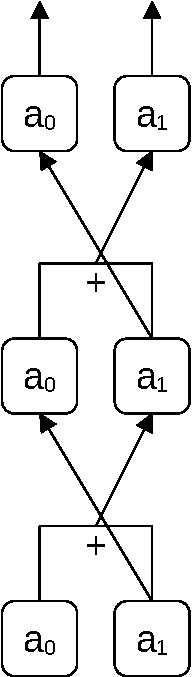
\includegraphics[width=.35\textwidth]{\recursiondir/figures/fibonacci-sm}
\end{subfigure}
\caption{PIL code for the Fibonacci sequence and the equivalent representation as a state machine with registers $a_0$ and $a_1$.}
\label{fig:Fibo-sm}
\end{figure}

The execution trace for the particular instance of this state machine (i.e., $a_0(g) = 1$ and $a_1(g) = 1$) is as follows:
\[
\begin{array}{|c|c|c|c|c|}
\hline
\multicolumn{5}{|c|}{\textbf{Execution Trace}} \\\hline
\textbf{Registers} & \boldsymbol{L_1} & \boldsymbol{L_{32}} & \boldsymbol{a_0} & \boldsymbol{a_1} \\\hline
\textbf{State 1} & {\color{green!50!black} 1} & {\color{green!50!black} 0} & {\color{green!50!black} 1} & {\color{red} 1} \\\hline
\textbf{State 2} & {\color{green!50!black} 0} & {\color{green!50!black} 0} & {\color{red} 1} & {\color{red} 2} \\\hline
\textbf{State 3} & {\color{green!50!black} 0} & {\color{green!50!black} 0} & {\color{red} 2} & {\color{red} 3} \\\hline
\vdots & \vdots & \vdots & \vdots & \vdots \\\hline
\textbf{State 31} & {\color{green!50!black} 0} & {\color{green!50!black} 1} & {\color{red} 1346269} & {\color{red} 2178309} \\\hline
\textbf{State 32} & {\color{green!50!black} 0} & {\color{green!50!black} 1} & {\color{red} 2178309} & {\color{green!50!black} 3524578} \\
\hline
\end{array}
\]

After the description of the circuit in PIL we can proceed to generate a valid eSTARK proof for this particular instance using \texttt{pil-stark}:
\begin{enumerate}
\item Populate the constant polynomials in the execution trace:
\begin{lstlisting}[style=termt]
$ mkdir -p build && node src/main_buildconst.js -o build/fibonacci.const

file Generated Correctly
\end{lstlisting}

\item Populate the committed polynomials in the execution trace:
\begin{lstlisting}[style=termt]
$ node src/main_buildcommit.js -i src/input.json -o build/fibonacci.commit

Result: 3524578
file Generated Correctly
\end{lstlisting}

\item Verify that the execution trace generated in the previous two steps is valid:
\begin{lstlisting}[style=termt]
$ node node_modules/pilcom/src/main_pilverifier.js build/fibonacci.commit -p src/fibonacci.pil -c build/fibonacci.const

PIL OK!!
\end{lstlisting}

\item Create a \texttt{starkstruct.json} file with the eSTARK parameters in the same directory:
\begin{lstlisting}[style=termt]
$ cat <<EOT > starkstruct.json
{
    "nBits": 5,
    "nBitsExt": 6,
    "nQueries": 64,
    "verificationHashType": "GL",
    "steps": [
        {"nBits": 6},
        {"nBits": 4},
        {"nBits": 2}
    ]
}
EOT
\end{lstlisting}

\item Generate the \texttt{starkinfo.json} file needed to generate the eSTARK:
\begin{lstlisting}[style=termt]
$ node node_modules/pil-stark/src/main_genstarkinfo.js -p src/fibonacci.pil -s src/starkstruct.json -i build/starkinfo.json

files Generated Correctly
\end{lstlisting}

\item Preprocess the state machine:
\begin{lstlisting}[style=termt]
$ node node_modules/pil-stark/src/main_buildconsttree.js -c build/fibonacci.const -p src/fibonacci.pil -s src/starkstruct.json -t build/fibonacci.consttree -v build/fibonacci.verkey.json

files Generated Correctly
\end{lstlisting}

\item Generate the eSTARK proof:
\begin{lstlisting}[style=termt]
$ node node_modules/pil-stark/src/main_prover.js -m build/fibonacci.commit -c build/fibonacci.const -t build/fibonacci.consttree -p src/fibonacci.pil -s build/starkinfo.json -o build/fibonacci.proof.json -z build/fibonacci.zkin.json -b build/fibonacci.public.json

files Generated Correctly
\end{lstlisting}

\item Finally, verify the proof:
\begin{lstlisting}[style=termt]
$ node node_modules/pil-stark/src/main_verifier.js -p src/fibonacci.pil -s build/starkinfo.json -v build/fibonacci.verkey.json -o build/fibonacci.proof.json -b build/fibonacci.public.json

Verification Ok!!
\end{lstlisting}
\end{enumerate}


%%%%%%%%%%%%%%%%%%%%%%%%%%%%%%%%%%%%%%%%%%%%%%%%%%%%%%
\subsection{Depth 0: Circom + PIL-STARK}

In this section, we show how to generate an eSTARK proof over the Fibonacci circuit written in Circom directly.
\begin{enumerate}
\item Compile the circuit:
\begin{lstlisting}[style=termt]
$ mkdir -p build && circom src/fibonacci.circom --O1 --prime goldilocks --r1cs --wasm -o build

template instances: 1
non-linear constraints: 0
linear constraints: 31
public inputs: 1
public outputs: 1
private inputs: 1
private outputs: 0
wires: 34
labels: 35
\end{lstlisting}
Notice how in this case the goldilocks prime field was chosen instead of the prime field over which is defined the BN128 elliptic curve (the default field in Circom). This is because the conversion of a circuit written in Circom to a state machine written in PIL is only defined, for the moment, over the goldilocks field.

\item Create a \texttt{input.json} file with the inputs for our circuit in the same directory:
\begin{lstlisting}[style=termt]
$ cat <<EOT > input.json
  {"a0": 1, "a1": 1}
  EOT
\end{lstlisting}

\item Compute the witness for our inputs:
\begin{lstlisting}[style=termt]
$ snarkjs wc build/fibonacci_js/fibonacci.wasm src/input.json build/fibonacci.wtns

out = 3524578
\end{lstlisting}

\item Now that we have computed the witness (or more precise, the R1CS) we convert the R1CS representation of the circuit to an equivalent PlonK representation of the same circuit:
\begin{lstlisting}[style=termt]
$ node node_modules/pil-stark/src/main_plonksetup.js -r build/fibonacci.r1cs -p build/fibonacci.pil -e build/fibonacci.exec -c build/fibonacci.const

files Generated Correctly
\end{lstlisting}
The output state machine written in PIL is the following:
\begin{pil}
constant %N = 2**6;

namespace Global(%N);
    pol constant L1;
    pol constant L2;

namespace PlonkCircuit(%N);
    pol constant S[3];
    pol constant Qm, Ql, Qr, Qo, Qk;
    pol commit a[3];

    public pub0 = a[0](0);
    public pub1 = a[0](1);
    Global.L1 * (a[0] - :pub0) = 0;
    Global.L2 * (a[0] - :pub1) = 0;

// Normal plonk ecuations
    pol a01 = a[0]*a[1];
    Qm*a01 + Ql*a[0] + Qr*a[1] + Qo*a[2] + Qk = 0;

// Connection equations
    {a[0], a[1], a[2]} connect {S[0], S[1], S[2]};
\end{pil}

This process also outputs a file containing the constant polynomials generated during the conversion.

\item Populate the committed polynomials in the execution trace:
\begin{lstlisting}[style=termt]
$ node node_modules/pil-stark/src/main_plonkexec.js -w build/fibonacci.wtns -p build/fibonacci.pil -e build/fibonacci.exec -m build/fibonacci.commit

file Generated Correctly
\end{lstlisting}

\item Verify that the execution trace generated in the previous two steps is valid:
\begin{lstlisting}[style=termt]
$ node node_modules/pilcom/src/main_pilverifier.js build/fibonacci.commit -p build/fibonacci.pil -c build/fibonacci.const

PIL OK!!
\end{lstlisting}

\item Create a \texttt{starkstruct.json} file with the eSTARK parameters in the same directory:
\begin{lstlisting}[style=termt]
$ cat <<EOT > starkstruct.json
{
    "nBits": 6,
    "nBitsExt": 7,
    "nQueries": 64,
    "verificationHashType": "BN128",
    "steps": [
        {"nBits": 7},
        {"nBits": 5},
        {"nBits": 3}
    ]
}
EOT
\end{lstlisting}
Importantly, the number of bits needs to be increased from $5$ to $6$ due to the overhead of the R1CS to PlonK transformation (see the output state machine).

Now, we can proceed as in the previous example to generate the eSTARK.

\item Generate the \texttt{starkinfo.json} file needed to generate the eSTARK:
\begin{lstlisting}[style=termt]
$ node node_modules/pil-stark/src/main_genstarkinfo.js -p build/fibonacci.pil -s src/starkstruct.json -i build/starkinfo.json

files Generated Correctly
\end{lstlisting}

\item Preprocess the state machine:
\begin{lstlisting}[style=termt]
$ node node_modules/pil-stark/src/main_buildconsttree.js -c build/fibonacci.const -p build/fibonacci.pil -s src/starkstruct.json -t build/fibonacci.consttree -v build/fibonacci.verkey.json

files Generated Correctly
\end{lstlisting}

\item Generate the eSTARK proof:
\begin{lstlisting}[style=termt]
$ node node_modules/pil-stark/src/main_prover.js -m build/fibonacci.commit -c build/fibonacci.const -t build/fibonacci.consttree -p build/fibonacci.pil -s build/starkinfo.json -o build/fibonacci.proof.json -z build/fibonacci.zkin.json -b build/fibonacci.public.json

files Generated Correctly
\end{lstlisting}

\item Finally, verify the proof:
\begin{lstlisting}[style=termt]
$ node node_modules/pil-stark/src/main_verifier.js -p build/fibonacci.pil -s build/starkinfo.json -v build/fibonacci.verkey.json -o build/fibonacci.proof.json -b build/fibonacci.public.json

Verification Ok!!
\end{lstlisting}
\end{enumerate}

In the following sections, we expand beyond the previous two workflows by a combination of either \texttt{PIL-STARK} with itself or \texttt{PIL-STARK} with \texttt{SNARKjs}. 

%%%%%%%%%%%%%%%%%%%%%%%%%%%%%%%%%%%%%%%%%%%%%%%%%%%%%%
\subsection{Depth 1: Circom + PIL-STARK + SNARKjs}

We start by showing how to generate a SNARK proof that an eSTARK proof is valid over the statement represented in Circom:
\begin{enumerate}
\item Compile the circuit:
\begin{lstlisting}[style=termt]
$ mkdir -p build && circom src/fibonacci.circom --O1 --prime goldilocks --r1cs --wasm -o build

Everything went okay, circom safe
\end{lstlisting}

\item Create a \texttt{input.json} file with the inputs for our circuit in the same directory:
\begin{lstlisting}[style=termt]
$ cat <<EOT > input.json
    {"a0": 1, "a1": 1}
    EOT
\end{lstlisting}

\item Compute the witness for our inputs:
\begin{lstlisting}[style=termt]
$ snarkjs wc build/fibonacci_js/fibonacci.wasm src/input.json build/fibonacci.wtns

out = 3524578
\end{lstlisting}

\item Now that we have computed the witness (or more precise, the R1CS) we convert the R1CS representation of the circuit to an equivalent PlonK representation of the same circuit:
\begin{lstlisting}[style=termt]
$ node node_modules/pil-stark/src/main_plonksetup.js -r build/fibonacci.r1cs -p build/fibonacci.pil -e build/fibonacci.exec -c build/fibonacci.const

files Generated Correctly
\end{lstlisting}

\item Populate the committed polynomials in the execution trace:
\begin{lstlisting}[style=termt]
$ node node_modules/pil-stark/src/main_plonkexec.js -w build/fibonacci.wtns -p build/fibonacci.pil -e build/fibonacci.exec -m build/fibonacci.commit

file Generated Correctly
\end{lstlisting}

\item Verify that the execution trace generated in the previous two steps is valid:
\begin{lstlisting}[style=termt]
$ node node_modules/pilcom/src/main_pilverifier.js build/fibonacci.commit -p build/fibonacci.pil -c build/fibonacci.const

PIL OK!!
\end{lstlisting}

\item Create a \texttt{starkstruct.json} file with the eSTARK parameters in the same directory:
\begin{lstlisting}[style=termt]
$ cat <<EOT > starkstruct.json
{
    "nBits": 6,
    "nBitsExt": 7,
    "nQueries": 64,
    "verificationHashType": "BN128",
    "steps": [
        {"nBits": 7},
        {"nBits": 5},
        {"nBits": 3}
    ]
}
EOT
\end{lstlisting}

\item Generate the \texttt{starkinfo.json} file needed to generate the eSTARK:
\begin{lstlisting}[style=termt]
$ node node_modules/pil-stark/src/main_genstarkinfo.js -p build/fibonacci.pil -s src/starkstruct.json -i build/starkinfo.json

files Generated Correctly
\end{lstlisting}

\item Preprocess the state machine:
\begin{lstlisting}[style=termt]
$ node node_modules/pil-stark/src/main_buildconsttree.js -c build/fibonacci.const -p build/fibonacci.pil -s src/starkstruct.json -t build/fibonacci.consttree -v build/fibonacci.verkey.json

files Generated Correctly
\end{lstlisting}

\item Generate the eSTARK proof:
\begin{lstlisting}[style=termt]
$ node node_modules/pil-stark/src/main_prover.js -m build/fibonacci.commit -c build/fibonacci.const -t build/fibonacci.consttree -p build/fibonacci.pil -s build/starkinfo.json -o build/fibonacci.proof.json -z build/fibonacci.zkin.json -b build/fibonacci.public.json --proverAddr 0x7BAbF98C66454aF8a3C366F893f99EBa26a15c66

files Generated Correctly
\end{lstlisting}

\item We can verity that the proof is correct:
\begin{lstlisting}[style=termt]
$ node node_modules/pil-stark/src/main_verifier.js -p build/fibonacci.pil -s build/starkinfo.json -v build/fibonacci.verkey.json -o build/fibonacci.proof.json -b build/fibonacci.public.json

Verification Ok!!
\end{lstlisting}

\item Next, we generate an eSTARK verifier as a circuit written in Circom:
\begin{lstlisting}[style=termt]
$ node node_modules/pil-stark/src/main_pil2circom.js -p build/fibonacci.pil -s build/starkinfo.json -v build/fibonacci.verkey.json -o build/verifier.circom

file Generated Correctly
\end{lstlisting}
This will allow the recursivity to happen: if we generate a valid SNARK on input the previously generated eSTARK proof, then we will prove that the eSTARK proof is valid.

\item We compile the circuit using the circuits in \texttt{circuits.gl} needed to compile the eSTARK verifier circuit:
\begin{lstlisting}[style=termt]
$ circom build/verifier.circom --r1cs --wasm -l node_modules/pil-stark/circuits.bn128 -l node_modules/circomlib/circuits -o build

template instances: 465
non-linear constraints: 2123834
linear constraints: 0
public inputs: 0
public outputs: 1
private inputs: 14682
private outputs: 0
wires: 2125925
labels: 5010997
\end{lstlisting}

\item Create a \texttt{input.json} file with the inputs for our circuit in the same directory:
\begin{lstlisting}[style=termt]
$ cat <<EOT > input.json
  {"a0": 1, "a1": 1}
  EOT
\end{lstlisting}

\item Compute the witness for our inputs:
\begin{lstlisting}[style=termt]
$ snarkjs wc build/verifier_js/verifier.wasm build/fibonacci.zkin.json build/verifier.wtns

out = 3524578
\end{lstlisting}

\item Download sufficiently large ``powers of tau'' file:
\begin{lstlisting}[style=termt]
$ wget https://hermez.s3-eu-west-1.amazonaws.com/powersOfTau28_hez_final_16.ptau -O build/powersOfTau.ptau
\end{lstlisting}

\item Preprocess the circuit:
\begin{lstlisting}[style=termt]
$ snarkjs pks build/verifier.r1cs build/powersOfTau.ptau build/fibonacci.zkey

[INFO]  snarkJS: Reading r1cs
[INFO]  snarkJS: Plonk constraints: 2
[INFO]  snarkJS: Setup Finished
\end{lstlisting}

\item Export the verification key for the verification of the proof:
\begin{lstlisting}[style=termt]
$ snarkjs zkev build/veirifer.zkey build/veirifer-vk.json

[INFO]  snarkJS: EXPORT VERIFICATION KEY STARTED
[INFO]  snarkJS: > Detected protocol: plonk
[INFO]  snarkJS: EXPORT VERIFICATION KEY FINISHED
\end{lstlisting}

\item Generate the PlonK proof:
\begin{lstlisting}[style=termt]
$ snarkjs pkp build/veirifer.zkey build/veirifer.wtns build/veirifer.proof.json build/veirifer.public.json
\end{lstlisting}

\item Finally, verify the proof:
\begin{lstlisting}[style=termt]
$ snarkjs pkv build/veirifer-vk.json build/veirifer.public.json build/veirifer.proof.json

[INFO]  snarkJS: OK!
\end{lstlisting}
\end{enumerate}



%%%%%%%%%%%%%%%%%%%%%%%%%%%%%%%%%%%%%%%%%%%%%%%%%%%%%%
\subsection{Unlimited Depth with PIL-STARK}

In this section, we show how to generate an eSTARK proof that an eSTARK proof is valid over the Fibonacci sequence written in PIL. However, the same workflow can be repeated over and over to obtain an unlimited depth proof composition. As shown in the previous section, this unlimited eSTARK composition can always be ended up with a final SNARK. 

The following workflow exhibits the full power of the \texttt{PIL-STARK} and \texttt{SNARKjs} tool stack. 
\begin{enumerate}
\item Populate the constant polynomials in the execution trace:
\begin{lstlisting}[style=termt]
$ mkdir -p build && node src/main_buildconst.js -o build/fibonacci.const

file Generated Correctly
\end{lstlisting}

\item Populate the committed polynomials in the execution trace:
\begin{lstlisting}[style=termt]
$ node src/main_buildcommit.js -i src/input.json -o build/fibonacci.commit

Result: 3524578
file Generated Correctly
\end{lstlisting}

\item Verify that the execution trace generated in the previous two steps is valid:
\begin{lstlisting}[style=termt]
$ node node_modules/pilcom/src/main_pilverifier.js build/fibonacci.commit -p src/fibonacci.pil -c build/fibonacci.const

PIL OK!!
\end{lstlisting}

\item Create a \texttt{starkstruct.json} file with the eSTARK parameters in the same directory:
\begin{lstlisting}[style=termt]
$ cat <<EOT > fibonacci.starkstruct.json
{
    "nBits": 5,
    "nBitsExt": 6,
    "nQueries": 64,
    "verificationHashType": "GL",
    "steps": [
        {"nBits": 6},
        {"nBits": 4},
        {"nBits": 2}
    ]
}
EOT
\end{lstlisting}

\item Generate the \texttt{starkinfo.json} file needed to generate the eSTARK:
\begin{lstlisting}[style=termt]
$ node node_modules/pil-stark/src/main_genstarkinfo.js -p src/fibonacci.pil -s src/fibonacci.starkstruct.json -i build/starkinfo.json

files Generated Correctly
\end{lstlisting}

\item Preprocess the state machine:
\begin{lstlisting}[style=termt]
$ node node_modules/pil-stark/src/main_buildconsttree.js -c build/fibonacci.const -p src/fibonacci.pil -s src/fibonacci.starkstruct.json -t build/fibonacci.consttree -v build/fibonacci.verkey.json

files Generated Correctly
\end{lstlisting}

\item Generate the eSTARK proof:
\begin{lstlisting}[style=termt]
$ node node_modules/pil-stark/src/main_prover.js -m build/fibonacci.commit -c build/fibonacci.const -t build/fibonacci.consttree -p src/fibonacci.pil -s build/starkinfo.json -o build/fibonacci.proof.json -z build/fibonacci.zkin.json -b build/fibonacci.public.json

files Generated Correctly
\end{lstlisting}

\item We can verify that the proof is correct:
\begin{lstlisting}[style=termt]
$ node node_modules/pil-stark/src/main_verifier.js -p src/fibonacci.pil -s build/starkinfo.json -v build/fibonacci.verkey.json -o build/fibonacci.proof.json -b build/fibonacci.public.json

Verification Ok!!
\end{lstlisting}

\item Next, we generate an eSTARK verifier as a circuit in Circom:
\begin{lstlisting}[style=termt]
$ node node_modules/pil-stark/src/main_pil2circom.js -p src/fibonacci.pil -s build/starkinfo.json -v build/fibonacci.verkey.json -o build/verifier.circom

Verification Ok!!
\end{lstlisting}

\item We compile the circuit:
\begin{lstlisting}[style=termt]
$ circom --O1 --prime goldilocks --r1cs --wasm build/verifier.circom -l node_modules/pil-stark/circuits.gl -o build

Verification Ok!!
\end{lstlisting}

\item Compute the witness for our inputs:
\begin{lstlisting}[style=termt]
$ snarkjs wc build/verifier_js/verifier.wasm build/fibonacci.zkin.json build/verifier.wtns

out = 3524578
\end{lstlisting}

\item Convert the resulting circuit to a state machine:
\begin{lstlisting}[style=termt]
$ node node_modules/pil-stark/src/main_plonksetup.js -r build/verifier.r1cs -p build/verifier.pil -c build/verifier.const -e build/verifier.exec

files Generated Correctly
\end{lstlisting}

\item Populate the committed polynomials in the execution trace:
\begin{lstlisting}[style=termt]
$ node node_modules/pil-stark/src/main_plonkexec.js -w build/verifier.wtns -p build/verifier.pil -e build/verifier.exec -m build/verifier.commit

files Generated Correctly
\end{lstlisting}

\item Verify that the execution trace generated in the previous two steps is valid:
\begin{lstlisting}[style=termt]
$ node node_modules/pilcom/src/main_pilverifier.js build/verifier.commit -p build/verifier.pil -c build/verifier.const

PIL OK!!
\end{lstlisting}

\item Create a \texttt{verifier.starkstruct.json} file with the eSTARK parameters in the same directory:
\begin{lstlisting}[style=termt]
$ cat <<EOT > verifier.starkstruct.json
{
    "nBits": 16,
    "nBitsExt": 17,
    "nQueries": 64,
    "verificationHashType": "GL",
    "steps": [
        {"nBits": 17},
        {"nBits": 14},
        {"nBits": 10},
        {"nBits": 6}
    ]
}
EOT
\end{lstlisting}

Now, we can proceed as in the previous example to generate the eSTARK.

\item Generate the \texttt{starkinfo.json} file needed to generate the eSTARK:
\begin{lstlisting}[style=termt]
$ node node_modules/pil-stark/src/main_genstarkinfo.js -p build/verifier.pil -s src/verifier.starkstruct.json -i build/verifier.starkinfo.json

files Generated Correctly
\end{lstlisting}

\item Preprocess the state machine:
\begin{lstlisting}[style=termt]
$ node node_modules/pil-stark/src/main_buildconsttree.js -c build/verifier.const -p build/verifier.pil -s src/verifier.starkstruct.json -t build/verifier.consttree -v build/verifier.verkey.json

files Generated Correctly
\end{lstlisting}

\item Generate the eSTARK proof:
\begin{lstlisting}[style=termt]
$ node node_modules/pil-stark/src/main_prover.js -m build/verifier.commit -c build/verifier.const -t build/verifier.consttree -p build/verifier.pil -s build/verifier.starkinfo.json -o build/verifier.proof.json -z build/verifier.zkin.json -b build/verifier.public.json

files Generated Correctly
\end{lstlisting}

\item Finally, verify the proof:
\begin{lstlisting}[style=termt]
$ node node_modules/pil-stark/src/main_verifier.js -p build/verifier.pil -s build/verifier.starkinfo.json -v build/verifier.verkey.json -o build/verifier.proof.json -b build/verifier.public.json

Verification Ok!!
\end{lstlisting}
\end{enumerate}

As explained at the beginning, one can repeat this workflow by again generating an eSTARK verifier as a circuit written in Circom and following Steps 10-18, creating \texttt{starkstruct.json}'s files at each repetition.